\documentclass[11pt,a4paper]{article}
\usepackage{amsmath}
\usepackage{color}
\usepackage{csquotes}
\usepackage{enumitem}
\usepackage{fullpage}
\usepackage{gensymb}
\usepackage{graphicx}
\usepackage[colorlinks=true, linkcolor=blue]{hyperref}
\usepackage{pgfplots}
\usepackage{subfigure}
\usepackage{url}
\renewcommand{\arraystretch}{1.15} % line spacing in tabular

\begin{document}
\title{ENGN4528/6528: Computer Vision\\Term Project Report}
\author{Libo Yin (u5483742), Manab Chetia (u5492350)\\and Sakda Eamkulworapong(u5610617)\footnote{Libo is enrolled in ENGN4528. Manab and Sakda are enrolled in ENGN6528.}\\The Australian National University}
\maketitle

\section{Introduction}
\label{sec:intro}
The Household Object Recognition Challenge aims to train an image classifier that discriminates pictures of household objects, such as mugs, boxes, and toys. The given dataset contains 50 object classes, and four images are provided for each class. These four images are taken from different angles at the same well-illuminated object, with a clean, slightly reflective desktop background.

This challenge is characterised by its tiny dataset compared to the number of object classes. The PASCAL VOC 2007 dataset\cite{everingham2010pascal}, in contrast, provides 9963 images in 20 classes. Such scarcity renders popular methods such as convolutional neural network unusable. However, the fact that the images are almost noise-free means lower-level approaches can be taken. Our group managed to create two distinctively different final solutions. The first one is based on SIFT and hue histogram, and is designed specifically for this problem. In this solution, we also propose a new classifier that borrows ideas from the bag of visual words model and the nearest neighbour classifier. The second solution is a more generalized system based on GIST and neural network. Both systems are implemented in Python.

\section{SIFT + Hue Histogram Solution}
\subsection{SIFT Classification}
\label{sec:hist}

A common practice in SIFT-based image classification is the bag of visual words model. Its assumptions are stated as follows:
\begin{displayquote}
SIFT descriptors from all training images form an unknown number of clusters in the 128 dimensional vector space. These clusters have identical and diagonal covariance matrix.\footnote{An assumption of k-means clustering algorithm\cite{numrecipes3}. This is a very weak assumption. Given the first assumption satisfied, we suggest modelling extracted SIFT keypoint descriptors as a mixture of Gaussian.}
\end{displayquote}

Under these two assumptions, SIFT keypoint descriptors from all training images are clustered with k-means, and centroids are extracted as codewords. With nearest neighbour classification, SIFT keypoint descriptors from a test image are converted to a bag of codewords. An image classification problem is thus converted to a document classification problem.

While such method has been proven effective for large dataset, our empirical test has shown that it is unreliable for this particular problem. First, the number of clusters $K$ is hard to choose. Second, even with identical $K,$ the variance of classification accuracy is still large. (For details please refer to \hyperref[sec:bovw]{section~\ref{sec:bovw}}.) We believe that such instability is a consequence of the small dataset. With OpenCV, the entire dataset produces a total number of 45,296 SIFT keypoints. In a vector space with dimensionality as high as 128, it is not very likely that the aforementioned two assumptions shall be satisfied.

Here, we propose Set Nearest Neighbour (SNN), a classification algorithm for tasks where a datapoint is a set of independent vectors in a vector space. Denote the number of classes by $C,$ the number of training vectors per class by $N$ (for notational convenience, assume $N$ is a constant), the dimensionality of a vector by $D,$ and the number of vectors in the testing dataset by $M.$ Then the training dataset has shape $C\times N\times D,$ and the testing datapoint has shape $M\times D.$ We aim to create a \emph{C}-dimensional vector denoting the probability of the test datapoint (recall that it is a set of independent vectors) belonging to each class. This vector is collapsed from a 3-dimensional array of shape $M\times C\times N,$ where entry $(i,j,k)$ denotes the distance, according to some metric, from the \emph{i}-th vector of the test datapoint, to the \emph{k}-th vector in the training dataset of class \emph{j}. The third axis is collapsed by taking the minimum, followed by the first axis collapsed by taking the sum.

In other words, for each vector in the testing datapoint, we find, for each class, the minimum distance between that particular testing vector and any vector in the training dataset of this particular class. This step gives a \emph{C}-dimensional distance vector. And since all vectors in the testing datapoint are independent, we take the summation of all their corresponding distance vectors, which gives a \emph{C}-dimensional distance vector from the testing datapoint as a whole to each class. This vector is then turned into a discrete probability distribution by subtracting each entry from the largest value, and normalize such that all entries sum up to 1. Note that the result probability vector contains at least one zero, so $\epsilon$ has to be added to each entry before taking logarithm. This algorithm requires brute force calculation of distances, but for small, noise-free dataset, it provides exceptional accuracy and reliability.

For this particular problem, we extract 30 strongest SIFT keypoint descriptors from each image. Since the dataset is split such that exactly one image in each class is left as the test datapoint, $N=90,\ M=30, C=50,$ and $D=128.$ We choose Euclidean distance as the metric, following Lowe's original paper \cite{lowe1999object}. An efficient implementation of Euclidean distance is provided in \texttt{scipy.spatial.distance.cdist}. On 1000 random train/test splits, the SIFT + SNN classifier by itself produces an average accuracy of 0.9181, with a standard deviation of 0.0295. The classification takes approximately 0.8 second per split\footnote{Tested on a 2013 MacBook Pro with 2.0GHz processor. Parallel processing is not used in this project.}. Error analysis is shown in \hyperref[fig:sift_error]{figure~\ref{fig:sift_error}}.

\begin{figure}[htbp]
\centering
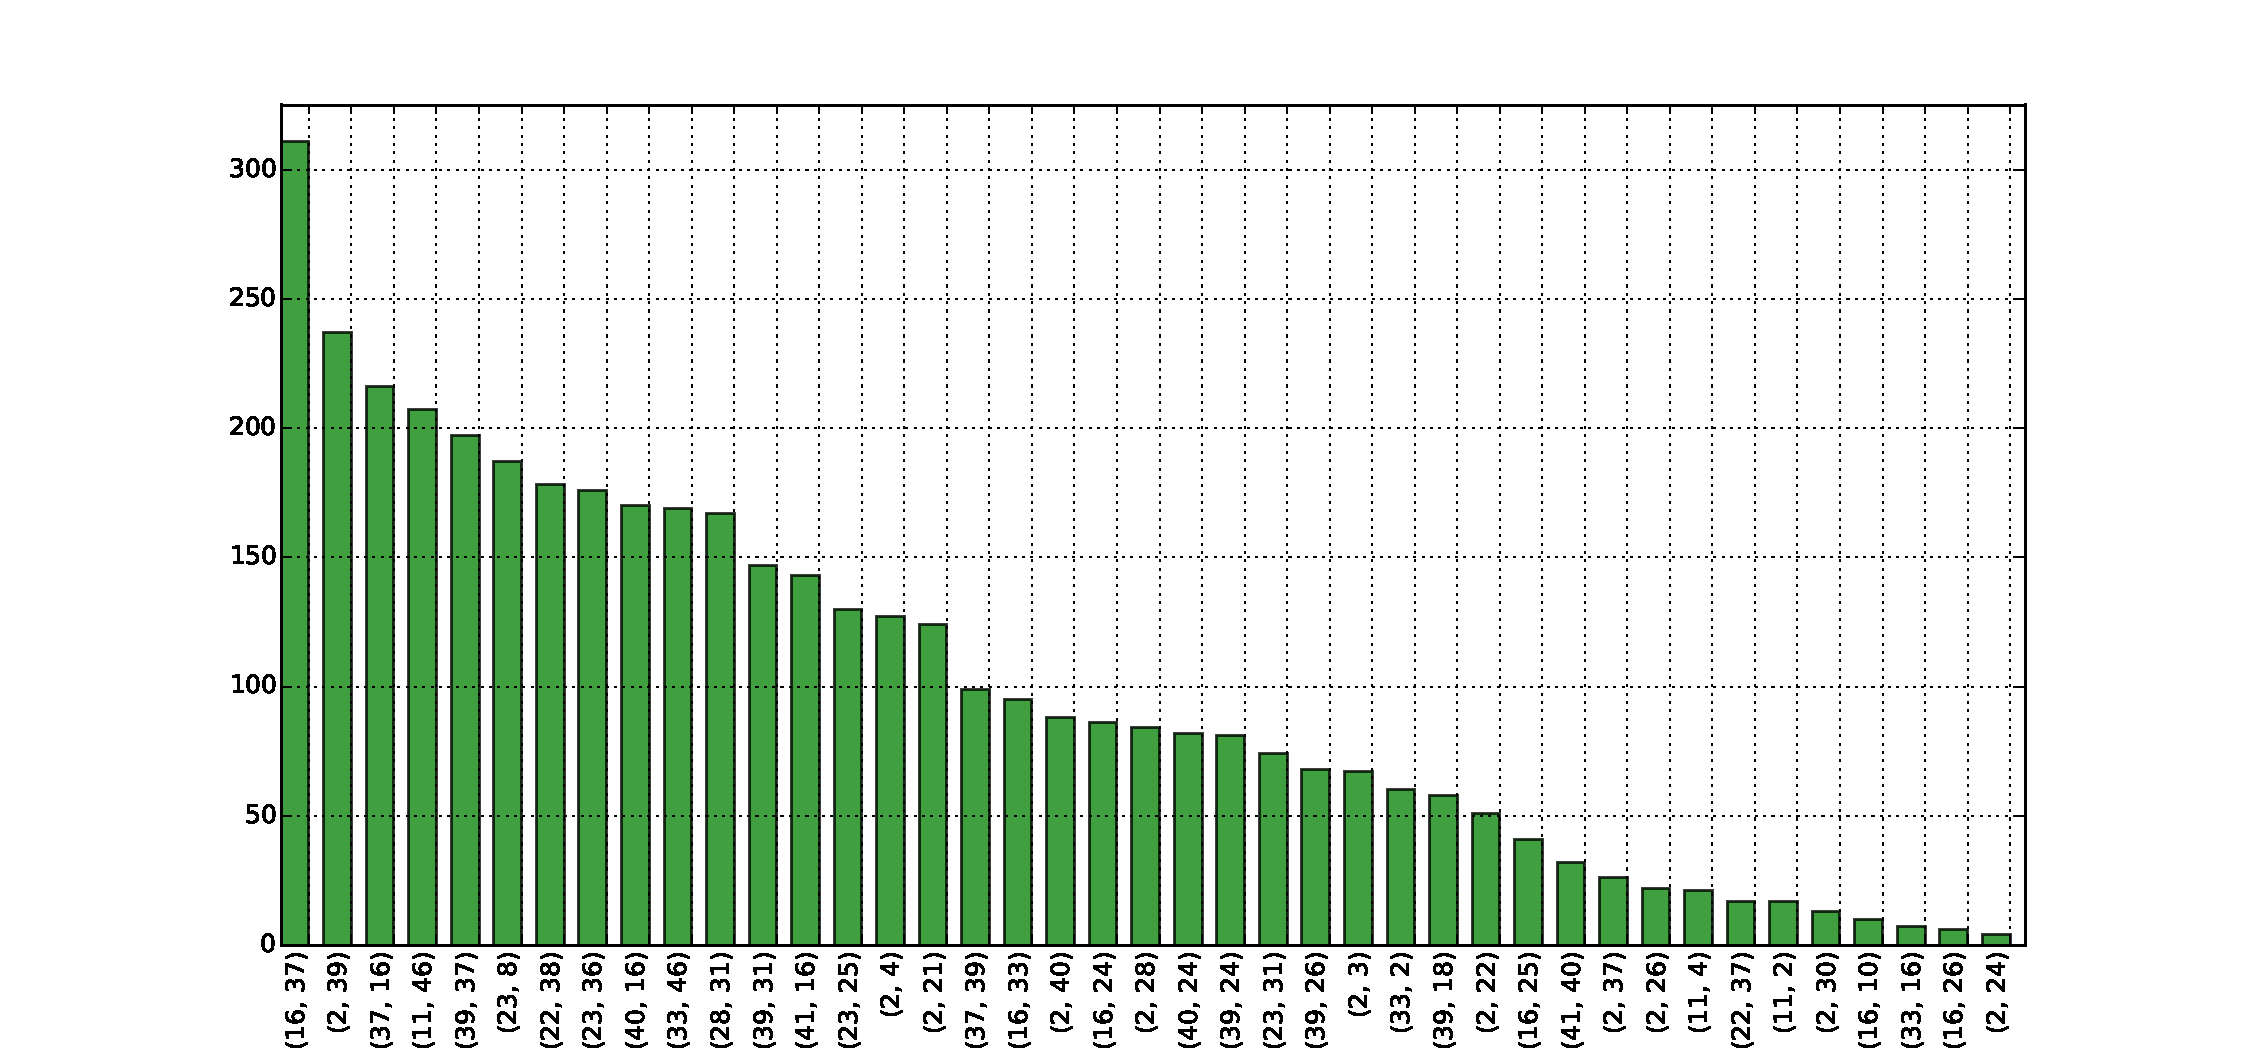
\includegraphics[scale=0.5]{sift_error.pdf}
\caption{Misclassification statistics of the SIFT + SNN classifier on 1000 random train/test splits. Labels under bars are in (\texttt{ground truth}, \texttt{prediction}) format. For example, the most frequent error is misclassifying image of class 16 as of class 37. The classifier made 4,095 misclassifications in total.}
\label{fig:sift_error}
\end{figure}

\subsection{Hue Histogram Classification}
\label{sec:hue_hist}

Many frequently misclassified images of the SIFT classifier are distinctively different in color. This is within expectation, as color and geometry should be independent features of an image, and an ideal classifier should take both into consideration.

Thanks to the fact that the SIFT + SNN classifier is a soft probabilistic classifier, we can easily combine it with any other classifiers in the same framework. Here, we propose the hue histogram intersection classifier. First, the hue channel of each image is binned into a 181-slot histogram\footnote{In OpenCV, the range of values in the hue channel of an 8-bit image is a closed interval [0, 180].}. Since the three training images of each class are only different in the angle from which the picture is taken, we assume that their difference in hue histogram is insignificant. Therefore, we define the hue histogram of a class as the mean of the hue histograms of the three training images in that particular class. Note that this is different to the SIFT + SNN classifier, in which SIFT keypoint descriptors from the three testing images of each class are considered independent. A testing image is classified by measuring the intersection between its own hue histogram and the hue histogram of each class:
\[K_{\cap}(\mathbf{a},\mathbf{b})=\sum_{i=1}^n\operatorname{min}(\mathbf{a}_i,\mathbf{b}_i)\]
where $\mathbf{a}$ and $\mathbf{b}$ are the two histograms with $n$ bins each. Like SNN, the hue histogram classifier is a soft classifier that produces a \emph{C}-dimensional probability vector. However, since histogram intersection is a similarity function instead of a metric, the normalization is carried out by first subtracting each entry in the similarity vector by the minimum, and normalize such that all entries add up to 1.

The result of the SIFT + SNN classifier and the hue histogram intersection classifier are combined by addition, with the log probability vector from the hue histogram intersection classifier multiplied by $w=0.35.$ Weight factor $w$ guarantees numerical stability, and its value is chosen by cross-validation. The combined classifier produces an average accuracy of 0.9896, with a standard deviation of 0.0130. The running time of the combined classifier remains at approximately 0.8 second per split, meaning that the running time of the hue histogram intersection classifier by itself is covered by noise. Discrimination analysis of the combined classifier is shown in \hyperref[fig:combined_disc]{figure~\ref{fig:combined_disc}}.

Although it is possible to combine more classifiers, we choose not to do so since parameter tuning will be difficult, and the model will be less elegant.

\begin{figure}[htbp]
\centering
\begin{subfigure}
\centering
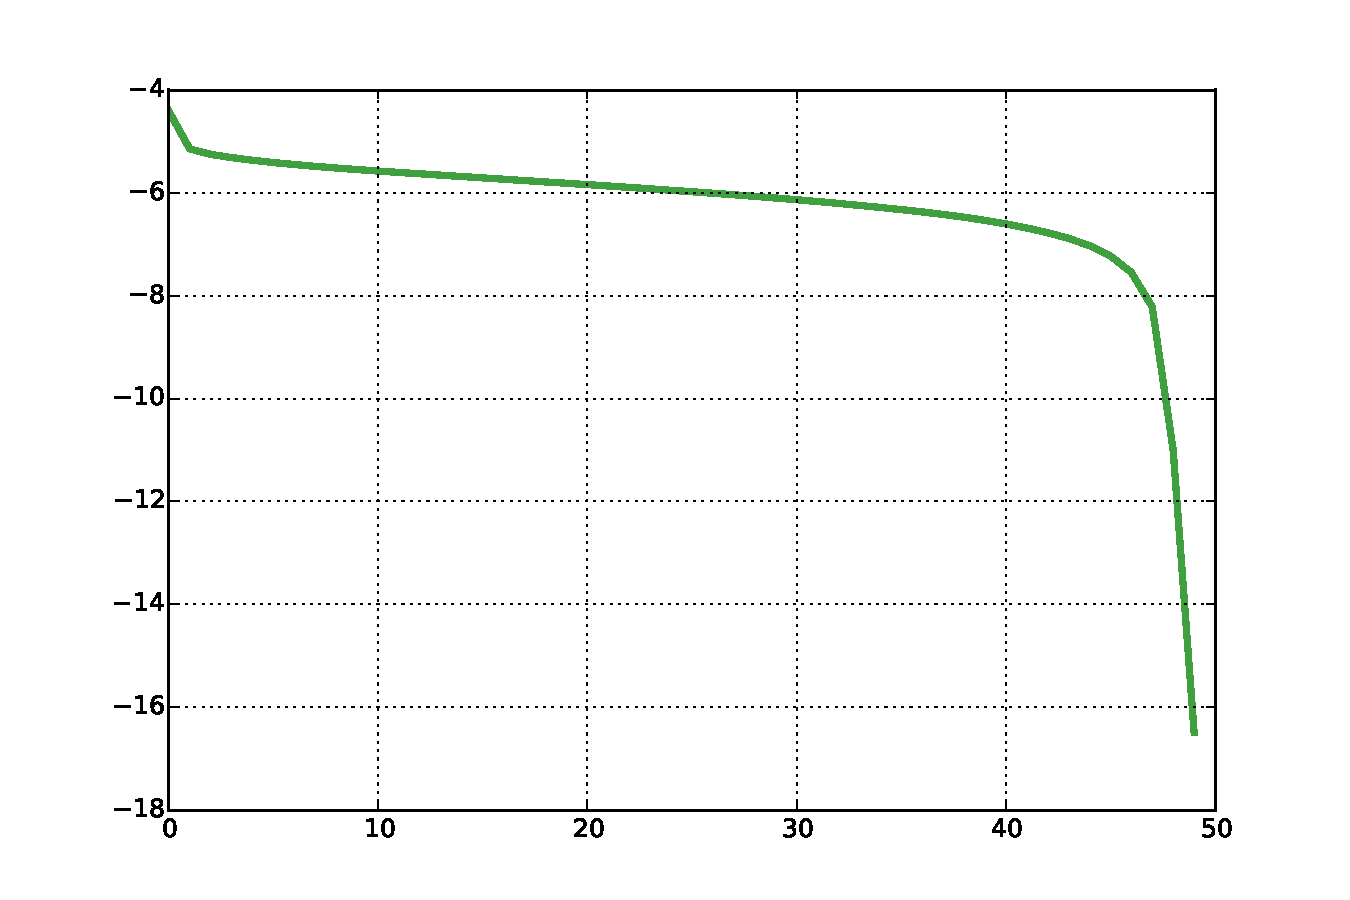
\includegraphics[scale=0.5]{combined_disc_all.pdf}
\end{subfigure}
\begin{subfigure}
\centering
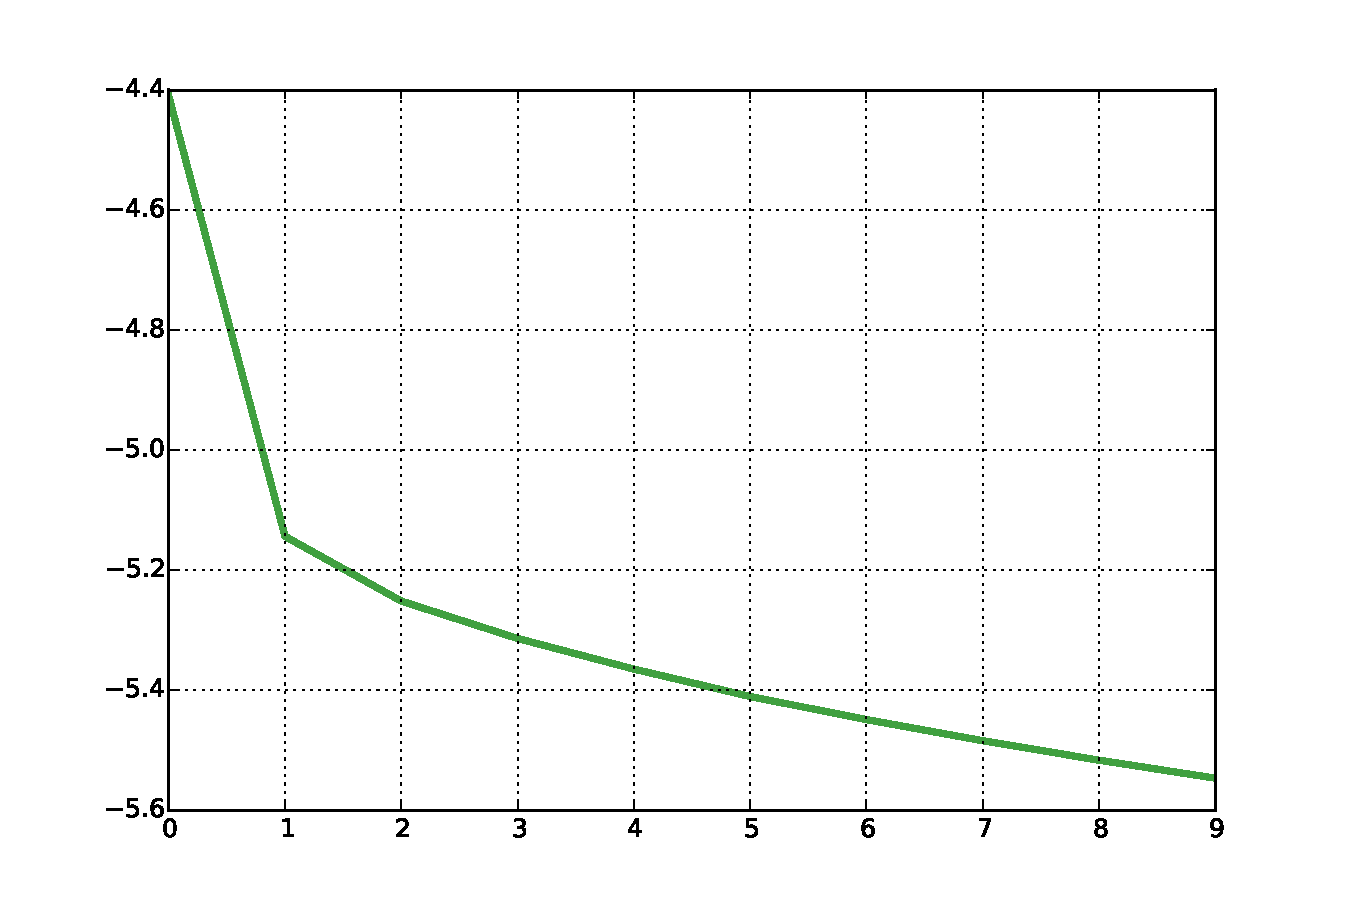
\includegraphics[scale=0.5]{combined_disc_top.pdf}
\end{subfigure}
\caption{Discrimination analysis for the combined classifier. Top: Sorted \emph{C}-dimensional probability vectors, averaged across all test images on 1000 random train/test splits. Horizontal axis is rank, and vertical axis is log probability. Most classes receive similar likelihood, hence the plateau in the middle. A few classes receive very low likelihood, due to the fact that normalization in both classifiers produce zeros. Bottom: Magnification of the top 10 classes in the top figure. It is clear that the leading class stands out from all others.}
\label{fig:combined_disc}
\end{figure}

\section{GIST + Neural Network Solution}

Currently, convolutional neural network is the state-of-the-art tool for image classification and object recognition. However, as mentioned in \hyperref[sec:intro]{section~\ref{sec:intro}}, training a convolutional neural network directly on the given dataset is infeasible due to its size. In this solution, we aim to approximate its performance by training a fully connected, feed-forward neural network on global features from an augmented dataset.

\subsection{Dataset Augmentation}

The original dataset contains 200 images in 50 object classes. In order to increase the size of dataset, we apply the following transformations to each image:
\begin{enumerate}[topsep=0.5em, itemsep=-0.5ex]
\item Rotation by $0\degree,\ 30\degree,\ 60\degree,\ 90\degree,\ 120\degree,\ 150\degree,\ 180\degree,\ 210\degree,\ 240\degree,\ 270\degree,\ 300\degree,$ and $330\degree.$
\item Gaussian blur with $\mu=0,\ \sigma=1.1.$
\item Gaussian noise with $\mu=0,\ \sigma=0.001.$
\item Darkening with $\gamma=1.5.$
\item Brightening with $\gamma=0.5.$
\end{enumerate}
The augmented dataset then contains 240 images per class\footnote{$12\text{ rotations}\times(4\text{ perturbation}+1\text{ identity})\times4\text{ original images per class}$}.

\subsection{Feature Extraction}

In \hyperref[sec:hist]{section~\ref{sec:hist}}, we demonstrated using a set of local SIFT keypoint descriptors as the global feature of an image. Here we use GIST\cite{oliva2001modeling}, a global feature by itself, to discriminate between classes. This choice is backed by the fact that all images in the given dataset have similar background, and there is only one object in each image. GIST summarises the gradient information (scales and orientation) for different parts of an image, and provides a low dimensional representation of the image's naturalness, openness, roughness, expansion, and ruggedness. The GIST descriptor of an image is calculated as follows:
\begin{enumerate}[topsep=0.5em, itemsep=-0.5ex]
\item Convolve an image with 20 Gabor filters at 8 orientations for two finer scales and 4
orientations for the coarser scales, giving rise to 20 feature maps.
\item Divide each feature map into 16 regions ($4\times4$ grid), then average the feature values
within each region for 3 colour channels.
\item Concatenate the $3\times16$ averaged values of all 20 feature maps, resulting in a $3\times16\times(8+8+4)=960$ dimensional vector.
\end{enumerate}

\subsection{Network Architecture}

The neural network has a fully connected, feed-forward structure, with one input layer, one hidden layer, and one output layer. The input layer contains 960 neurons, same as the dimensionality of a GIST descriptor. The output layer contains 50 neurons, corresponding to the number of object classes. The number of neurons in the hidden layer is chosen to be the average of the input layer and the output layer.

For the input layer and the hidden layer, the activation unit is rectified linear unit
(ReLU), which uses rectifier $f(x)=\operatorname{max}(0,x)$ as the activation function. ReLU is chosen since it induces sparsity in the hidden units, does not face gradient vanishing problem as with sigmoid and tanh, and is computationally efficient. The activation function for the output layer is softmax, a common practice for multi-class neural network classifier.

The loss function in our neural network is the cross entropy error, defined as:
\[E(\mathbf{o},\mathbf{t})=-\left(\mathbf{t}\cdot\log(\mathbf{o})+(\mathbf{1}-\mathbf{t})\cdot\log(\mathbf{1}-\mathbf{o})\right)\]
where $\mathbf{o}$ denotes the output distribution\footnote{The output of a softmax layer is a discrete probability distribution.}, and $\mathbf{t}$ denotes the ground truth, a vector with exactly one 1 entry and zero elsewhere. We choose the cross entropy error rather than the conventional squared error loss as it leads to faster training and better generalisation. Moreover, it is extremely sensitive to overconfident predictions\cite{mccaffrey2013cross}.

\subsection{Training and Testing}

The augmented dataset of $240\times50=12000$ images is randomly split into a training dataset of 9000 images and a testing dataset of 3000 images. Note that this is different from the testing scheme in the first solution, where the testing dataset is formed by randomly choosing exactly one of the four images from each class.

Both networks are trained with stochastic gradient descent (SGD) with Nesterov momentum and RMSprop\cite{hinton2012mini}. The parameters for SGD are: $\text{learning rate}=0.01,\ \text{decay}=10^{-6},$ and $\text{momentum}=0.9.$ For RMSprop, the parameters are: $\text{initial learning rate}=0.001,\ \text{decay rate}=0.9.$ On this problem, empirical experiments shows that RMSprop has a faster speed of convergence. This is because it modulates the learning rate of each weight based on the magnitudes of its gradients, which has an equalising effect. The comparison is shown in \hyperref[fig:sgd_rmsprop]{figure~\ref{fig:sgd_rmsprop}}.

\begin{figure}[htbp]
\centering
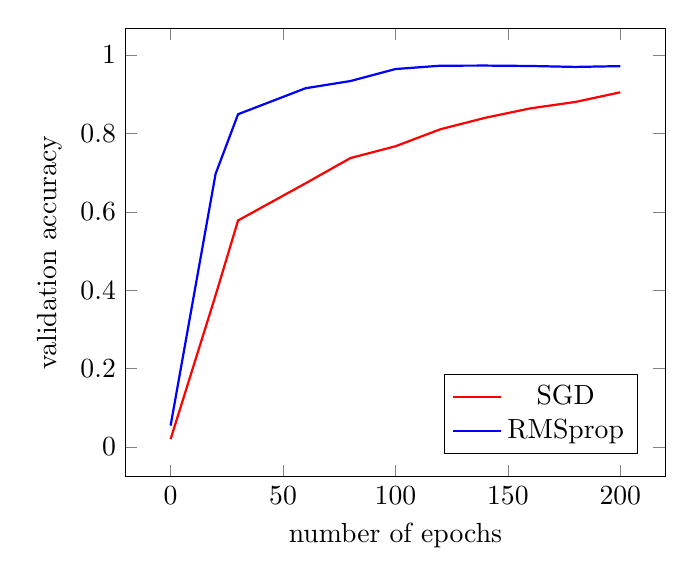
\begin{tikzpicture}[scale=1]
\begin{axis}[
	xlabel=number of epochs,
	ylabel=validation accuracy,
	legend style={at={(0.95,0.05)},anchor={south east}}]  % legend pos={south east} doesn't work
\addplot[color=red, style=thick] coordinates 
{
	(0, 0.02)
	(20, 0.387)
	(30, 0.578)
	(60, 0.6727)
	(80, 0.7373)
	(100, 0.7673)
	(120,0.8107)
	(140,0.84)
	(160,0.864)
	(180,0.8803)
	(200,0.905)
};
\addplot[color=blue, style=thick] coordinates 
{
	(0, 0.0547)
	(20, 0.6967)
	(30, 0.849)
	(60, 0.9153)
	(80, 0.9337)
	(100, 0.9643)
	(120,0.9728)
	(140,0.9731)
	(160,0.9721)
	(180,0.9697)
	(200,0.9717)
};
\legend{SGD,RMSprop}
\end{axis}
\end{tikzpicture}
\caption{Comparison of convergence speed of SGD and RMSprop}
\label{fig:sgd_rmsprop}
\end{figure}

To prevent overfitting, we introduce a dropout rate of 0.2 in the hidden layer. That is, with probability of 0.2, a hidden unit is set to 0. A dropout rate of 0.2 has also been tested in the input layer, but it lead to slower convergence and was hence removed.

With a batch size of 20 and 120 epochs of training, the classifier produced an accuracy of 97.32\%. With other aspects unchanged, we also tried reducing the dimensionality of input vectors from 960 to 400 with PCA (in which case the input layer has 400 neurons), and the classifier produced an accuracy of 96.6\%.

\section{Project Timeline}

During the entire lifetime of project, we used the GitHub Issues page\footnote{\url{https://github.com/liboyin/horc/issues}} to track unsolved problems, enhancements in progress, as well as personal timelines. Important events are listed in the following table. Note that different solutions may have different testing schemes.

\begin{table}[htbp]
\centering
\begin{tabular}{r|c|l}
Date & Member & Event\\
\hline
Mar 27 & All & Submission of proposal\\
Apr 13 & Libo & 20 SIFT + nearest neighbour: 80\% accuracy\\
Apr 15 & Manab & Root-SIFT + nearest neighbour: 75\% accuracy\\
Apr 24 & Libo & 20 SIFT + SNN: 91\% accuracy\\
Apr 25 & Sakda & Tested Shackenberg's Minimal bag of visual words classifier:\\
 & & 60\% accuracy\\
Apr 29 & Manab & GIST + nearest neigbour: 84\% accuracy\\
Apr 30 & Manab & GIST + SVM on polynomial kernel: 80\% accuracy\\
May 2 & Libo & Soft probabilistic classifiers\\
May 2 & Libo & 25 SIFT + SNN + hue histogram: 95\% accuracy\\
May 3 & Sakda & SIFT match without filter or threshold: 80\% accuracy\\
May 3 & Sakda & SIFT match with fileter and threshold: 90\% accuracy\\
May 10 & Sakda & Custom bag of visual words classifier: 85\% accuracy\\
May 12 & Manab & GIST + neural network: 84\% accuracy\\
May 12 & Manab & Dataset augmentation\\
May 12 & Manab & GIST + neural network + SGD on augmented dataset:\\
 & & 94.4\% accuracy\\
May 20 & Manab & GIST + PCA + neural network + RMSprop on augmented\\
 & & dataset: 96.6\% accuracy\\
May 25 & Libo & Map-reduce paradigm\\
May 25 & Libo & 30 SIFT + SNN + hue histogram, with tuned parameter:\\
 & & 98.9\% accuracy\\
May 26 & Manab & GIST + neural network + DropOut + RMSprop on augmented\\
 & & dataset: 97.32\% accuracy\\
May 27 & All & Project demo\\
\end{tabular}
\end{table}

\section{Conclusion}

With the given dataset, we managed to create two distinctively different solutions. Both of them exploit the fact that images are noise-free, and both of them have achieved an accuracy higher than 95\%. Listed in the appendix are a few of our other attempts. They are unable to produce satisfactory classification accuracy on the given dataset, but have nonetheless inspired us on our final solutions.

\clearpage
\appendix
\section{Other Attempts}
\subsection{SIFT on Hue Channel}

As mentioned in \hyperref[sec:hue_hist]{section~\ref{sec:hue_hist}}, color and geometry are independent features of an image. This is not entirely true. Theoretically, extracting SIFT keypoints from the hue channel should allow a feature that combines color and geometry information. Unfortunately, with OpenCV, some images in the given dataset are only able to produce as few as 1 SIFT keypoint from its hue channel, making this feature unusable.

\subsection{Classification with kNN and SVM}

In early stage of this project, we tried classifying image features directly with distance-based classifiers. Assuming SIFT keypoint descriptors are representative to their classes, we extracted 25 strongest SIFT keypoint descriptors from each image. For a testing image, each SIFT keypoint descriptor is classified with 4-nearest-neighbour classifier, and the overall class of that testing image is decided by voting. Despite the fact that the aforementioned model assumption is clearly violated, this classifier produced an accuracy of 0.82. Replacing set of local features with a global feature GIST, the accuracy improved slightly to 0.84.

We also tested SVM as classifier on the same features. Unlike kNN, which uses Euclidean distance as metric, SVM uses polynomial kernel with $\text{degree}=3$ instead of RBF. This choice is made by cross-validation. The SVM classifier produced a similar accuracy, but runs considerably faster than kNN since it avoids brute force calculation of pairwise distance.

\subsection{Bag of Visual Words}
\label{sec:bovw}

Our bag of visual words classifier is based on \cite{shackenbergbovw}. In the training stage, we extract 10 strongest SIFT keypoint descriptors from each training image\footnote{The train/test split is the same as in the first solution.}. We did not use all SIFT keypoint descriptors for speed reasons. These descriptors are clustered with k-means, and the centroids are extracted as codewords. Each class is then converted into a histogram of frequency, where each bin is a codeword.

Likewise, in the testing stage, 10 strongest SIFT keypoint descriptors are extracted from each image. These descriptors are classified to codewords with nearest neighbour on Euclidean distance. With the occurrence frequency of codewords obtained, the testing image is represented as a histogram, which is further classified by nearest neighbour on Euclidean distance.

The impact of number of clusters $K$ on prediction accuracy is shown in \hyperref[fig:bovw_exp]{figure~\ref{fig:bovw_exp}}. Note that the accuracy has a standard deviation of at least 0.025. The reason of such a high standard deviation has been discussed in \hyperref[sec:hist]{section~\ref{sec:hist}}. By setting $\text{cluster factor}=1.5$ and choosing top 80 SIFT feature descriptors from each training image, this classifier can reach an accuracy of 80-85\%.

\begin{figure}[htbp]
\centering
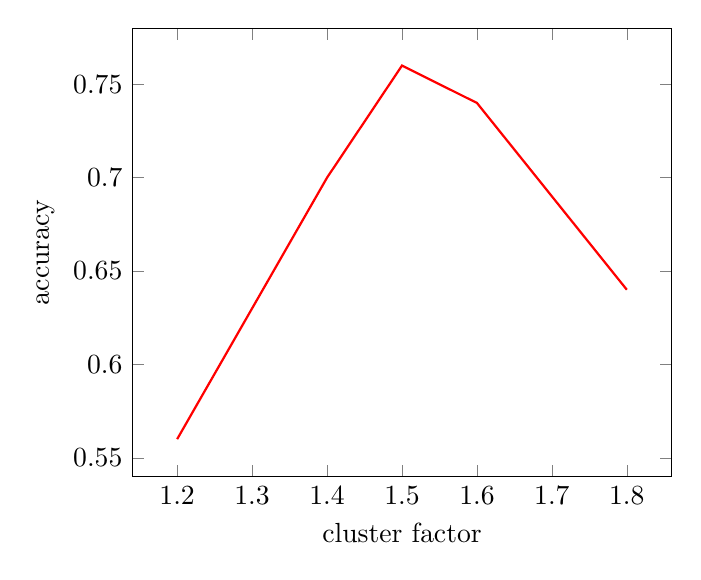
\begin{tikzpicture}[scale=1]
\begin{axis}[xlabel=cluster factor, ylabel=accuracy]
\addplot[color=red, style=thick] coordinates 
{
	(1.2, 0.56)
	(1.4, 0.70)
	(1.5, 0.76)
	(1.6, 0.74)
	(1.8, 0.64)
};
\end{axis}
\end{tikzpicture}
\caption{Impact of $K$ on classification accuracy. $K=\text{cluster factor}\times\text{number of classes}.$}
\label{fig:bovw_exp}
\end{figure}

\newpage
\subsection{SIFT Match}

We assume that images of the same class have more matching SIFT keypoints than images of different classes. With \texttt{siftmatch}, each testing image is compared to all training images, and is classified to the class which provides the highest number of matches. This approach allows an accuracy of 80\%, with some misclassifications shown in \hyperref[fig:siftmatch_error]{Figure~\ref{fig:siftmatch_error}}.

By experiments, we found that specifying $\text{edge threshold}=12$ and applying a negative Gaussian filter\cite{Brahmbhatt,lindeberg1996scale}
\[
-\begin{bmatrix}
0.0113 & 0.0838 & 0.0113\\ 
0.0838 & 0.6193 & 0.0838\\ 
0.0113 & 0.0838 & 0.0113
\end{bmatrix}
\]
before extracting SIFT keypoints improves accuracy to 90\%. We believe that this filter has reached a balance between reducing noise and suppressing image details. A few examples are shown in \hyperref[fig:filter]{figure~\ref{fig:filter}} and \hyperref[fig:filter_error]{figure~\ref{fig:filter_error}}.

\begin{figure}[htbp]
    \centering
    \subfigure[33 matches on images of the same class.]{
        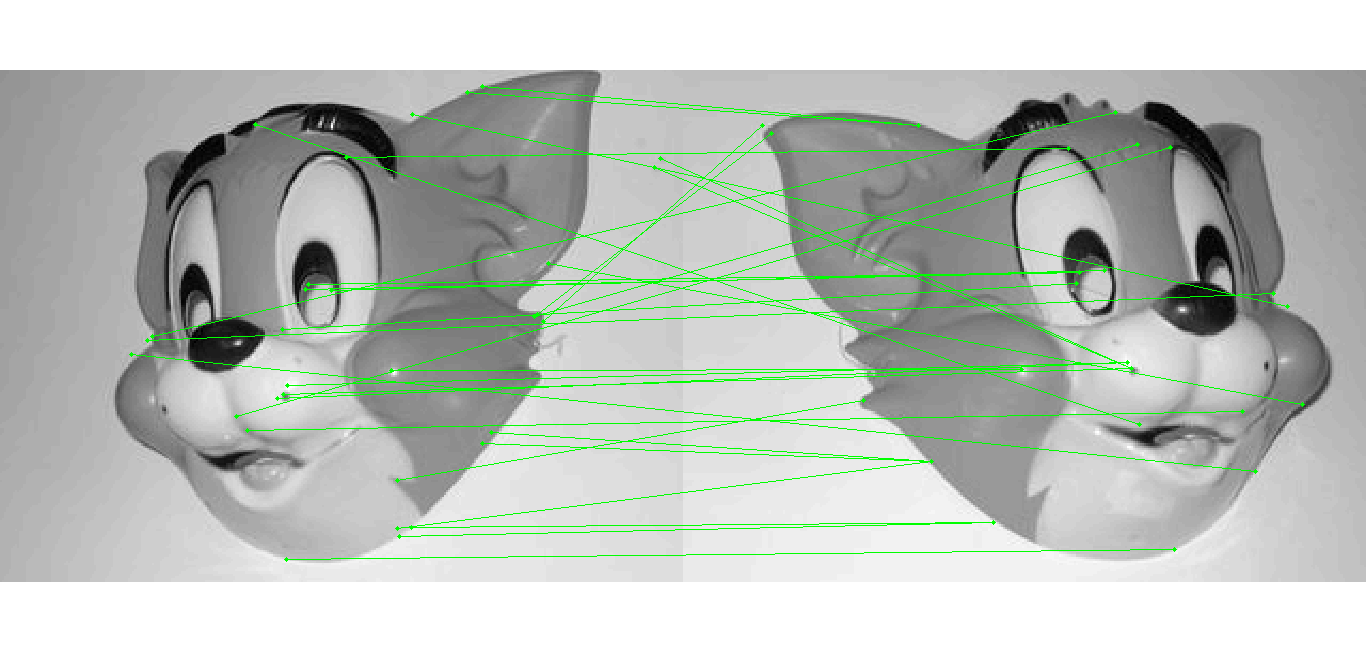
\includegraphics[scale=0.2]{toy_pair.png}
    }
    \subfigure[58 matches on images of different classes.]{
        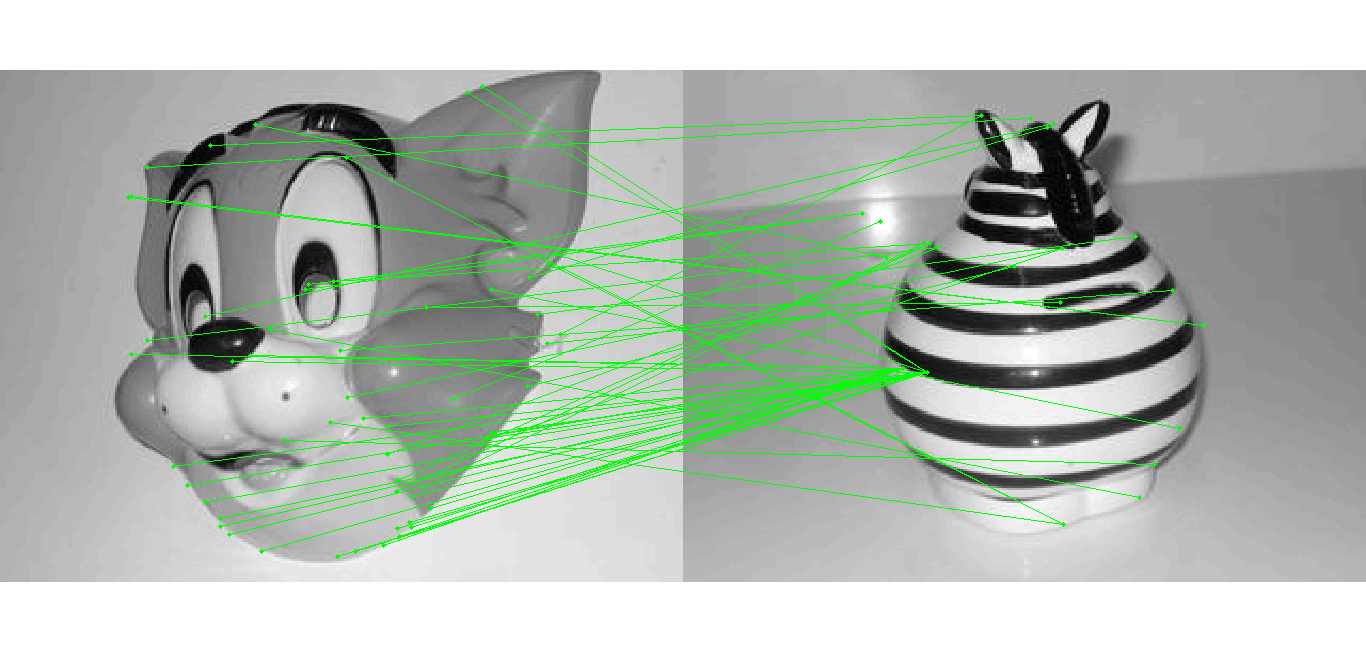
\includegraphics[scale=0.2]{toy_unpair.png}
    }
    \subfigure[31 matches on images of the same class.]{
        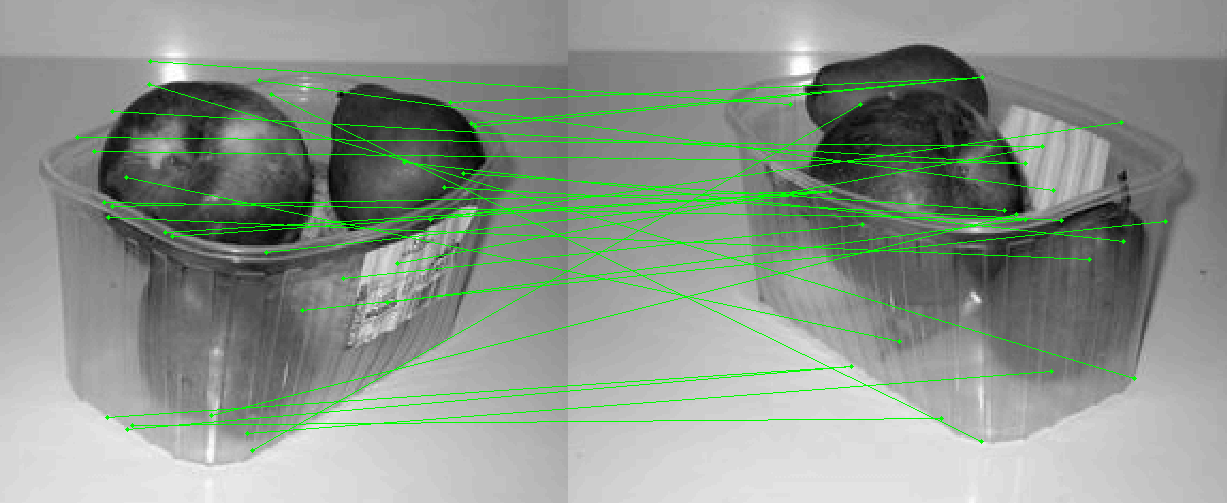
\includegraphics[scale=0.3]{fruits.png}
    }
    \subfigure[32 matches on images of different classes.]{
        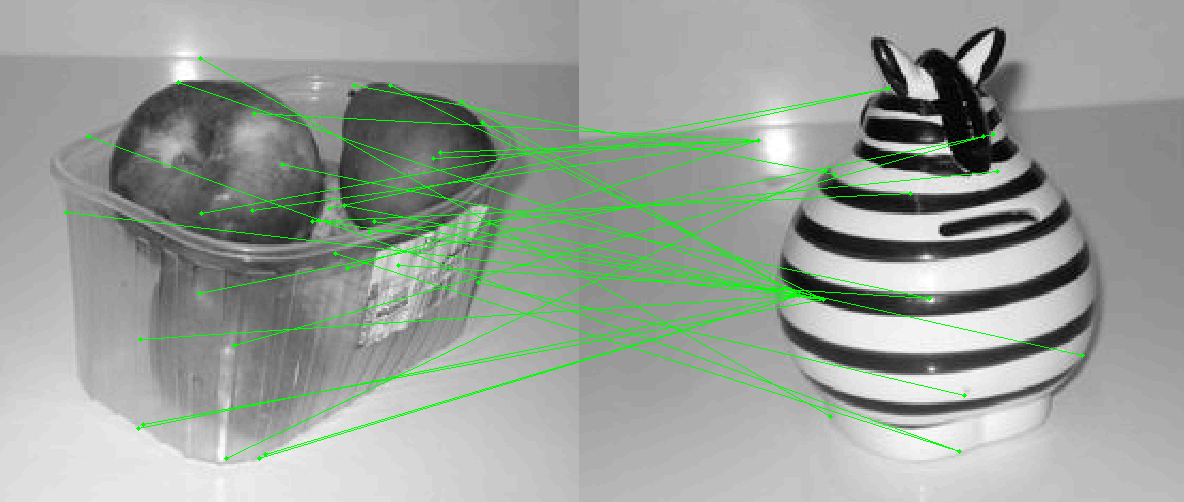
\includegraphics[scale=0.31]{fruit_toy.png}
    }
    \caption{Most misclassifications are on toys and fruits.}
    \label{fig:siftmatch_error}
\end{figure}

\begin{figure}[htbp]
    \centering
    \subfigure{
        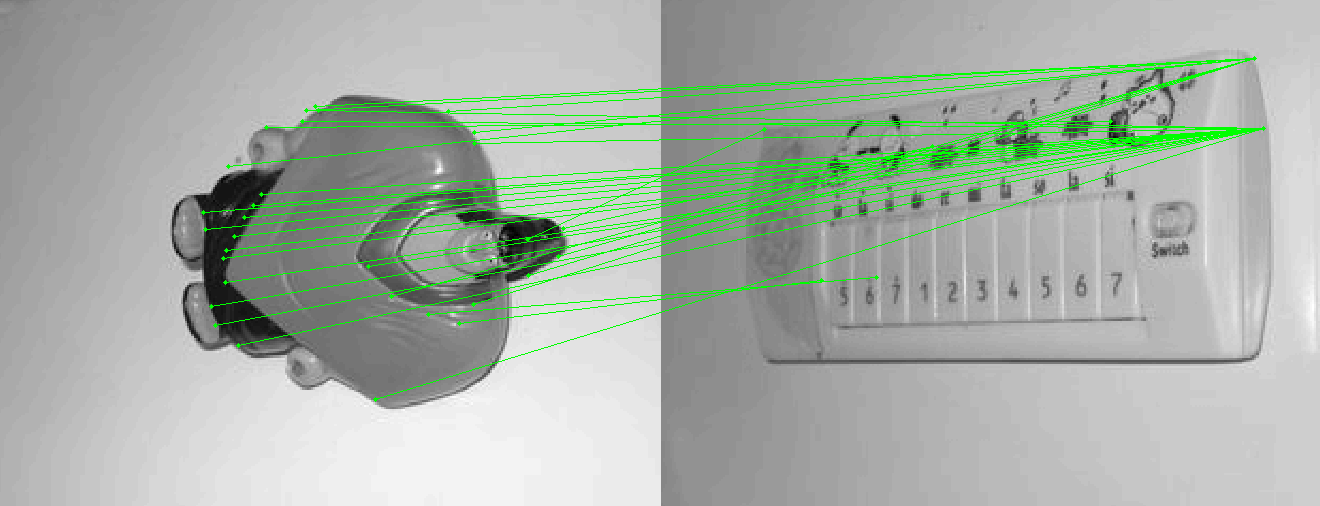
\includegraphics[scale=0.3]{no_filter.png}
    }
    \subfigure{
        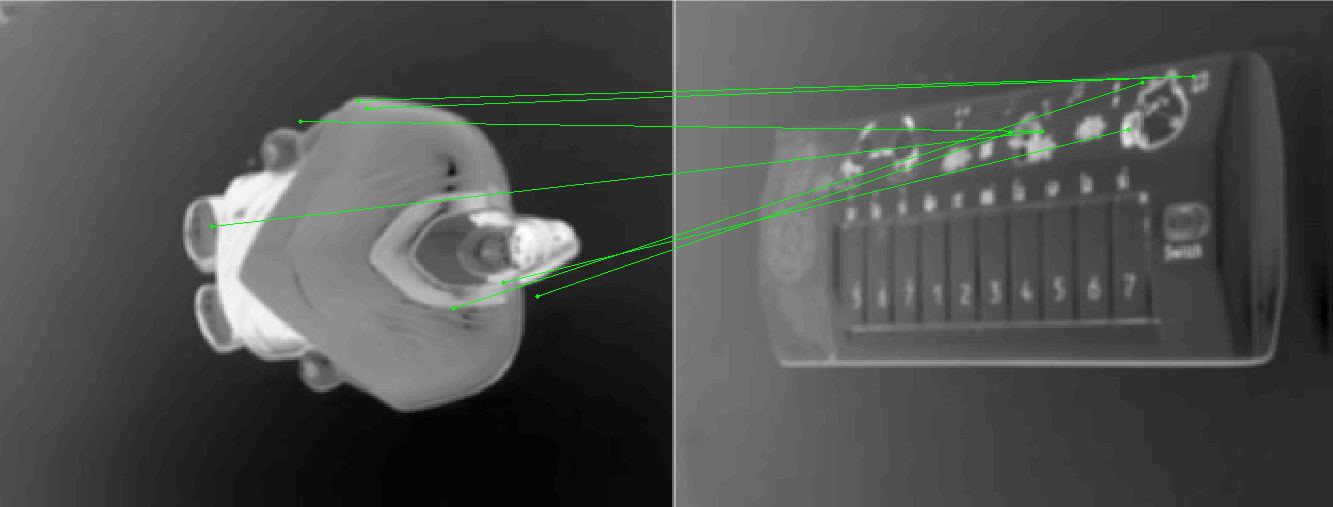
\includegraphics[scale=0.3]{filtered.png}
    }
    \caption{An example of SIFT match before and after filtering. Top: original images. Bottom: filtered images.}
    \label{fig:filter}
\end{figure}

\begin{figure} [htbp]
    \centering
    \subfigure{
        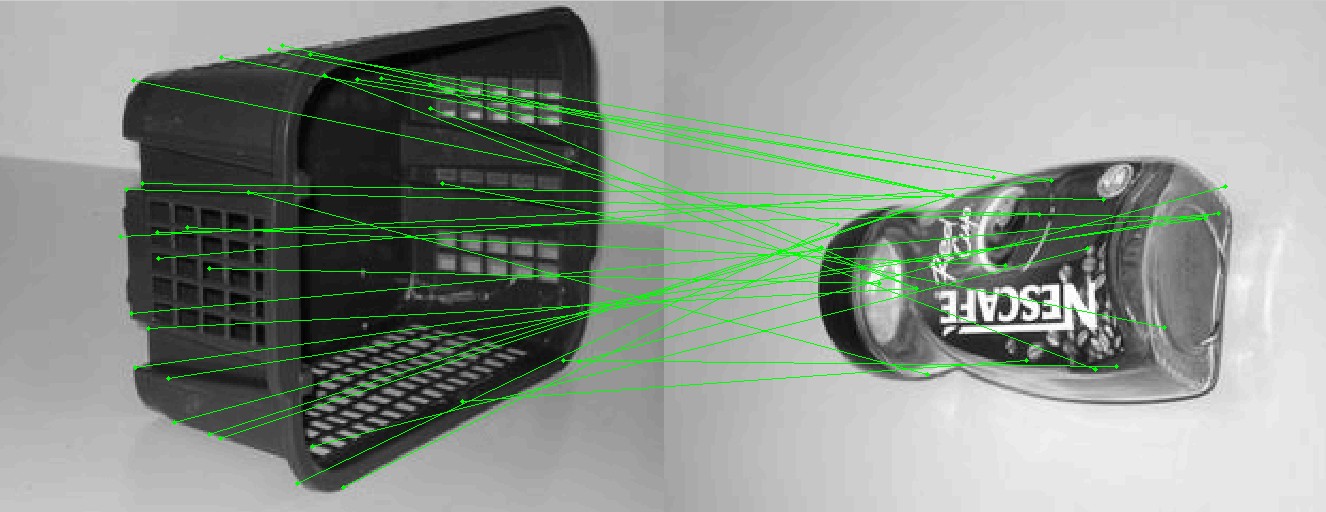
\includegraphics[scale=0.3]{no_filter1.png}
    }
    \subfigure{
        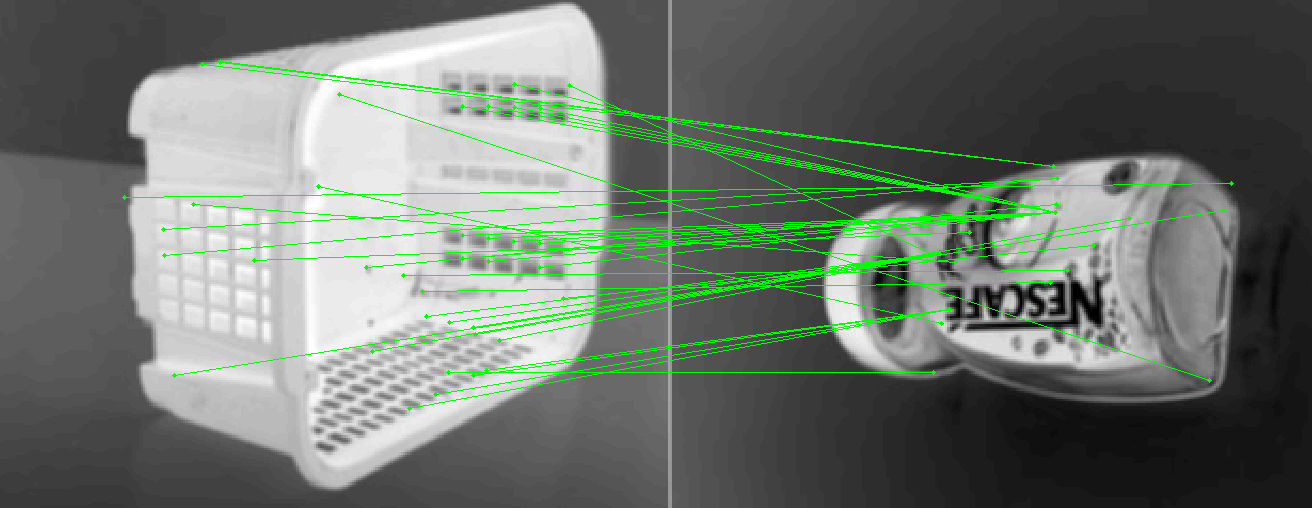
\includegraphics[scale=0.3]{filtered1.png}
    }
    \caption{On certain images, filtering leads to more matching SIFT keypoints. Top: original images. Bottom: filtered images.}
    \label{fig:filter_error}
\end{figure}

\clearpage
\bibliographystyle{plain}
\bibliography{Report}
\end{document}
